	The total power produced along this high speed machining was calculated as in the equation \ref{eq_power}, the values are shown on figure \ref{fig:totPower}.

	\begin{figure}[H]
		\centering
		\captionsetup{justification=centering}
		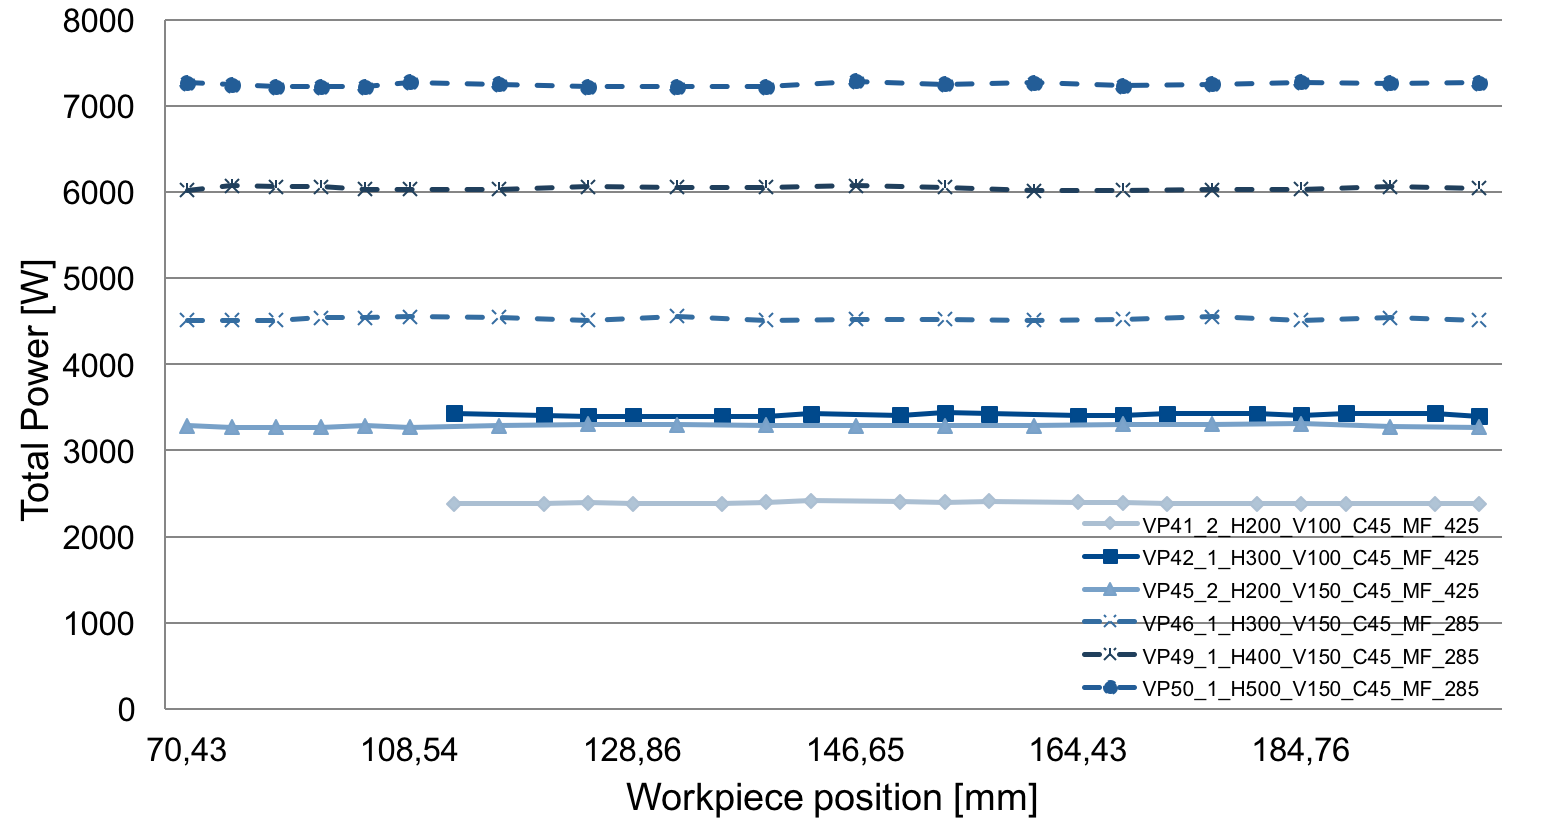
\includegraphics[scale=0.55]{Imagens/Total_power.png}
		\caption{Total power produced}
		\label{fig:totPower}
	\end{figure}

	As expected, the higher are the values of cutting velocity or depth of cut higher are the values of total power produced.
	For each experiment, the computational method was able to provide the thermal energy that goes to tool, chip and workpiece by means of energy balance. Then, it can be observed the thermal behavior of every area of interest along the workpiece position. The measurement starts when a reasonable area of the cutting zone reaches the minimum temperature. For cutting velocity of $150 m/min$ it starts earlier because the rate of heat production is higher than when the cutting velocity is $100 m/min$.

	\begin{figure}[H]
		\centering
		\captionsetup{justification=centering}
		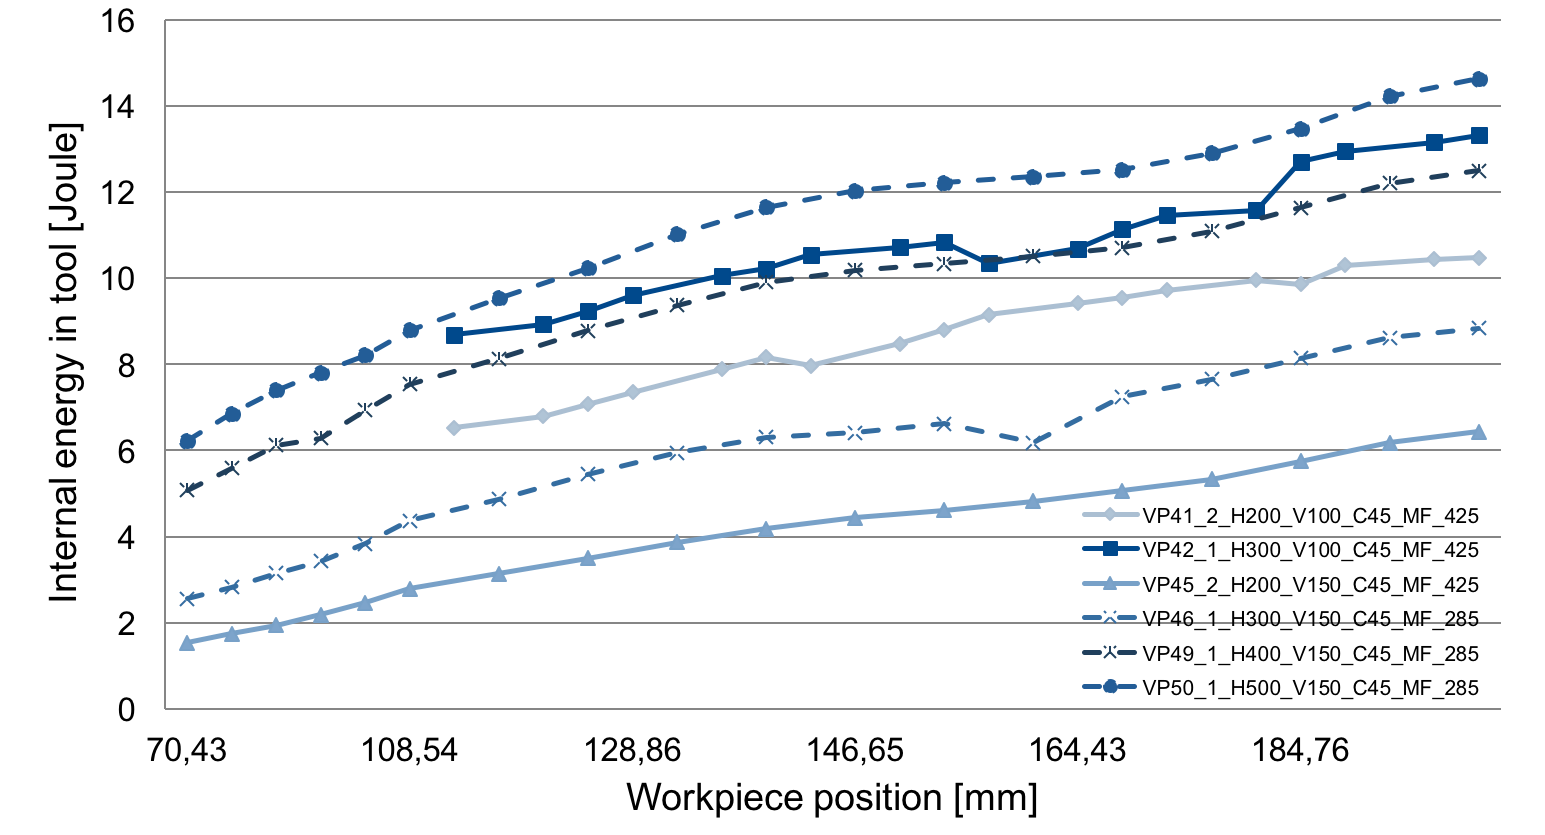
\includegraphics[scale=0.55]{Imagens/Inner_Energy.png}
		\caption{Inner energy of tool along workpiece position}
		\label{fig:innerTool}
	\end{figure}

	\begin{figure}[H]
		\centering
		\captionsetup{justification=centering}
		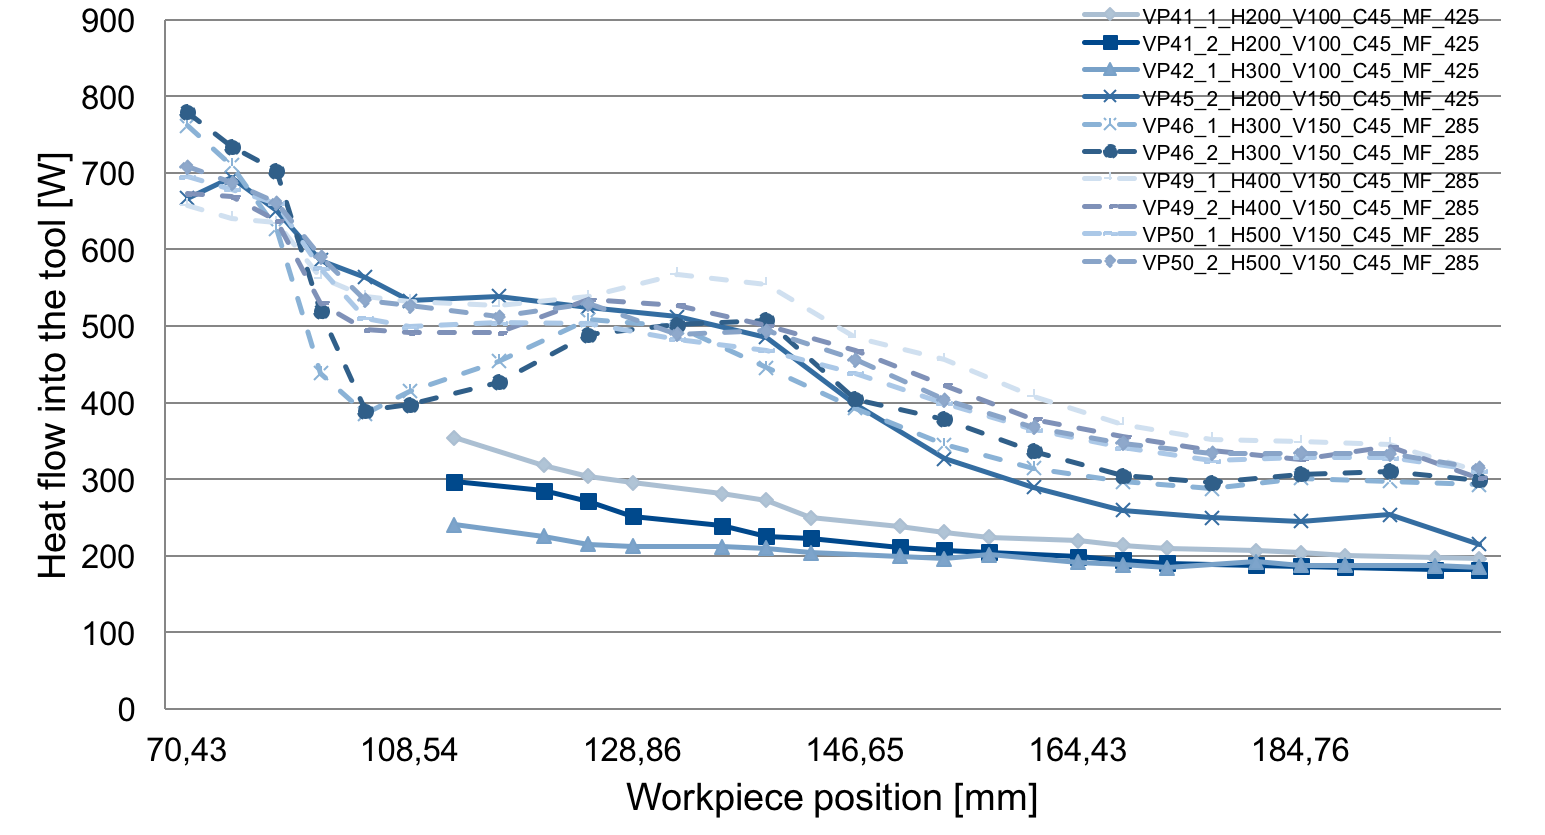
\includegraphics[scale=0.55]{Imagens/energyTool2.png}
		\caption{Heat flow into tool}
		\label{fig:hflowTool}
	\end{figure}

	As it can be observed on the previous figure \ref{fig:hflowTool}, the change rate of the inner energy of tool begins with a higher value than in the end of process. The rate starts to stabilize, indicating the beginning of the steady state. 

	To exemplify the results, it will be taken to represent the outcomes concerning heat partitions the experiment with cutting velocity $v_{c} = 150 m/min$ and depth of cut $a_{p} = 500 \mu m$. All the others experiments had approximately the same behavior during the cutting process.
	Concerning about the heat partition through tool, workpiece and the energy carried away by chip, their behaviors can be observed on the figure \ref{fig:hpartExp}. There is a slight decrement in the heat flow through tool, which it was expected due to the steady state as discussed before. As for the energy carried by chip, it may be noticed a slight increment.

	\begin{figure}[H]
		\centering
		\captionsetup{justification=centering}
		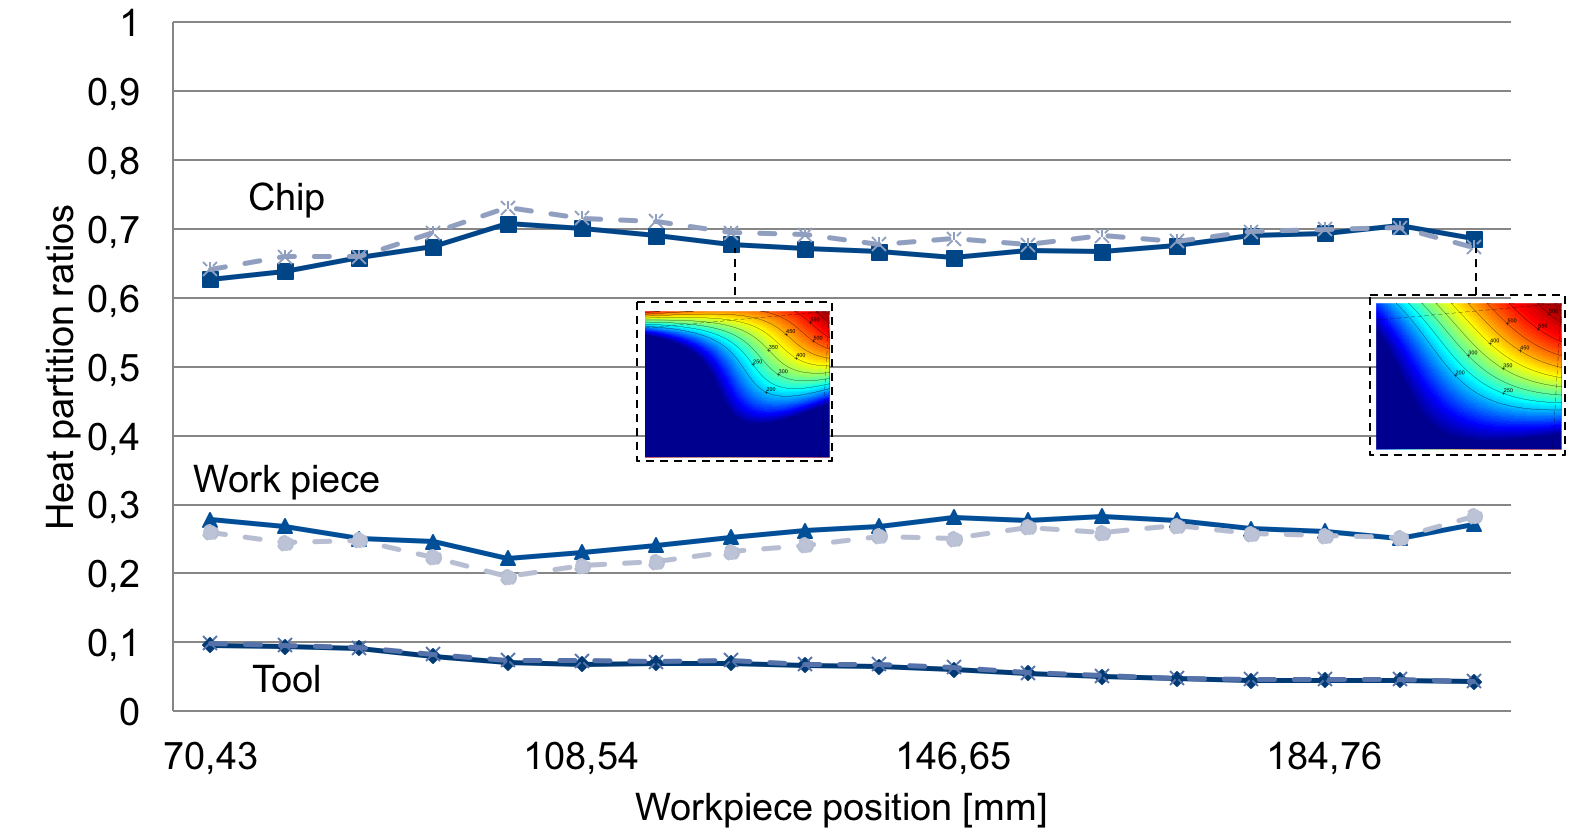
\includegraphics[scale=0.55]{Imagens/partition500150.png}
		\caption{Heat partition for experiment with a$_{p}$ = 500$\mu$m and v$_{c}$ = 150 m/min}
		\label{fig:hpartExp}
	\end{figure}

	It is important to highlight the total power produced during the cutting process, which has a significant value because of the high values of cutting velocity and force. Also, it must be noticed the amount of energy that goes to chip (figure \ref{fig:energyChip} and \ref{fig:hpartChip}). The chip takes around 70\% of the total energy produced, this fact may be explained due to the high temperatures that the region can reach and the high velocity of flowing.

	\begin{figure}[H]
		\centering
		\captionsetup{justification=centering}
		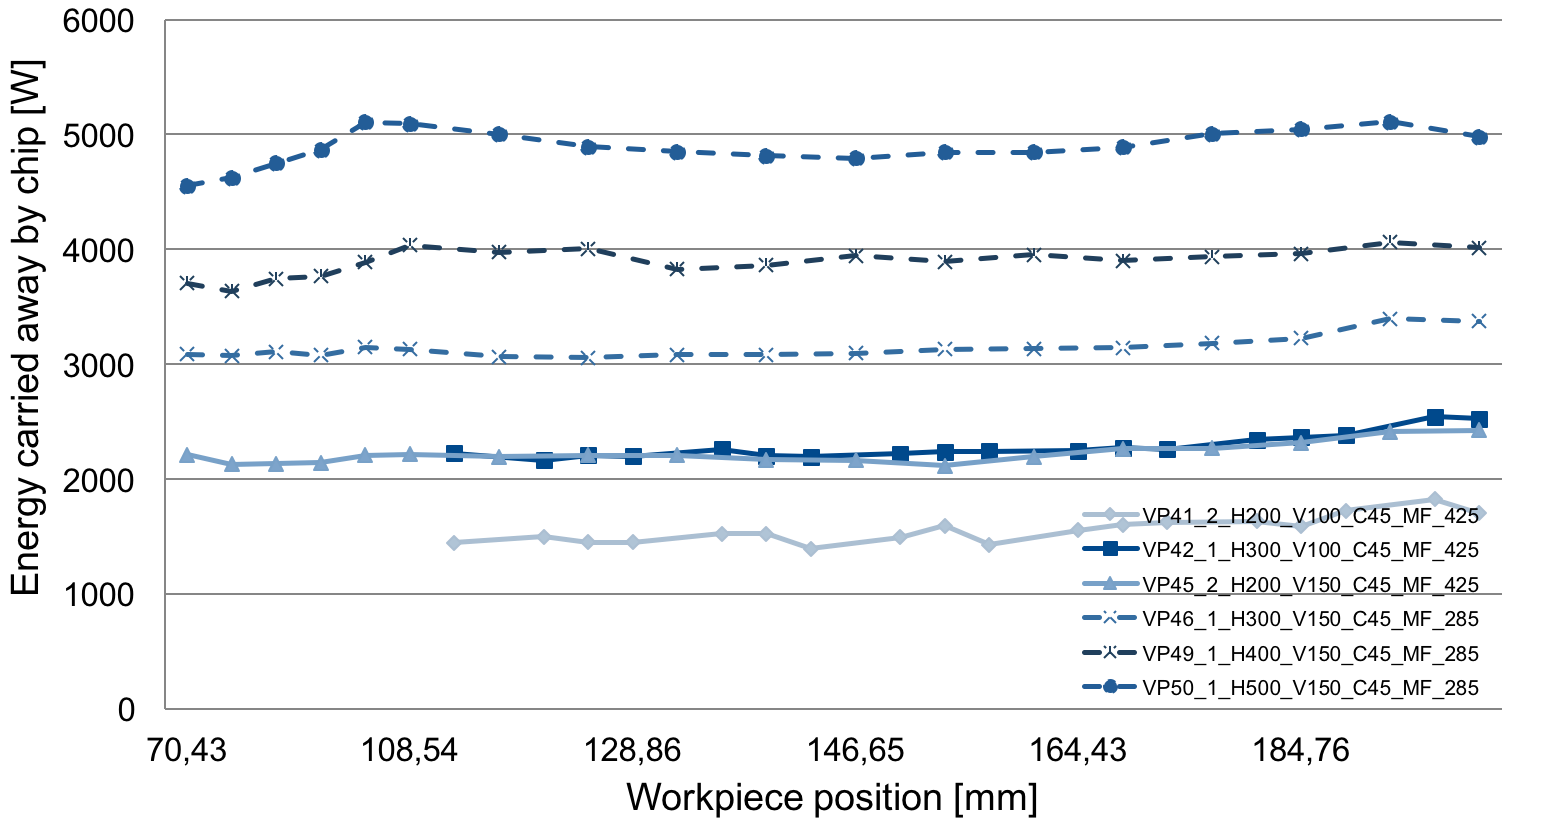
\includegraphics[scale=0.55]{Imagens/energyChip.png}
		\caption{Thermal energy into chip}
		\label{fig:energyChip}
	\end{figure}

	\begin{figure}[H]
		\centering
		\captionsetup{justification=centering}
		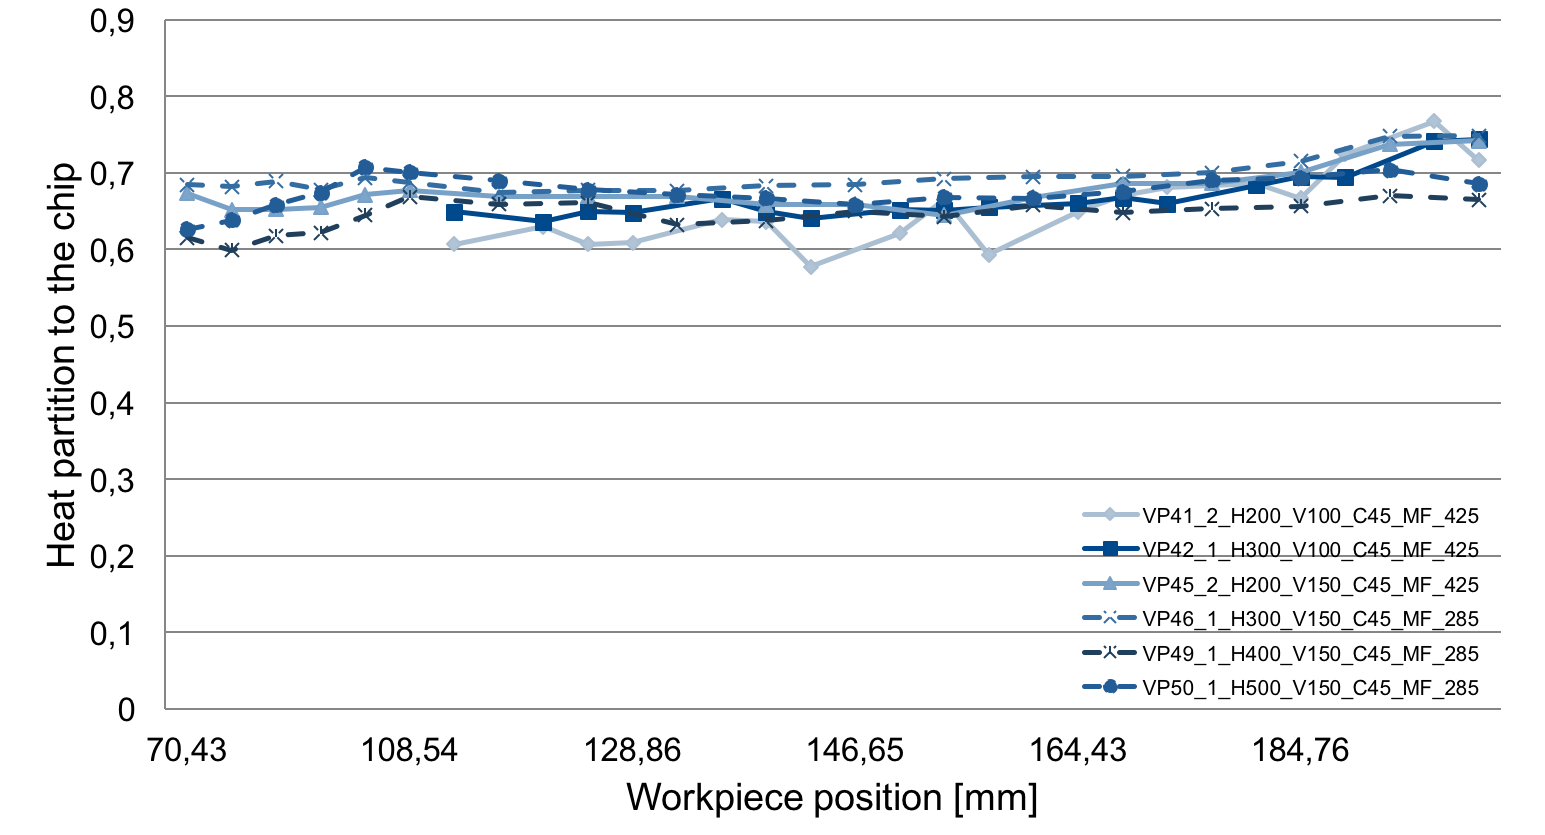
\includegraphics[scale=0.55]{Imagens/PartChip.png}
		\caption{Heat partition ratio for chip}
		\label{fig:hpartChip}
	\end{figure}

	As for the tool (figure \ref{fig:hpartTool}), the partition of energy reaches a much smaller range when close to the steady state. The values of the partition to tool in this stage goes from 4\% until 8\%.

	\begin{figure}[H]
		\centering
		\captionsetup{justification=centering}
		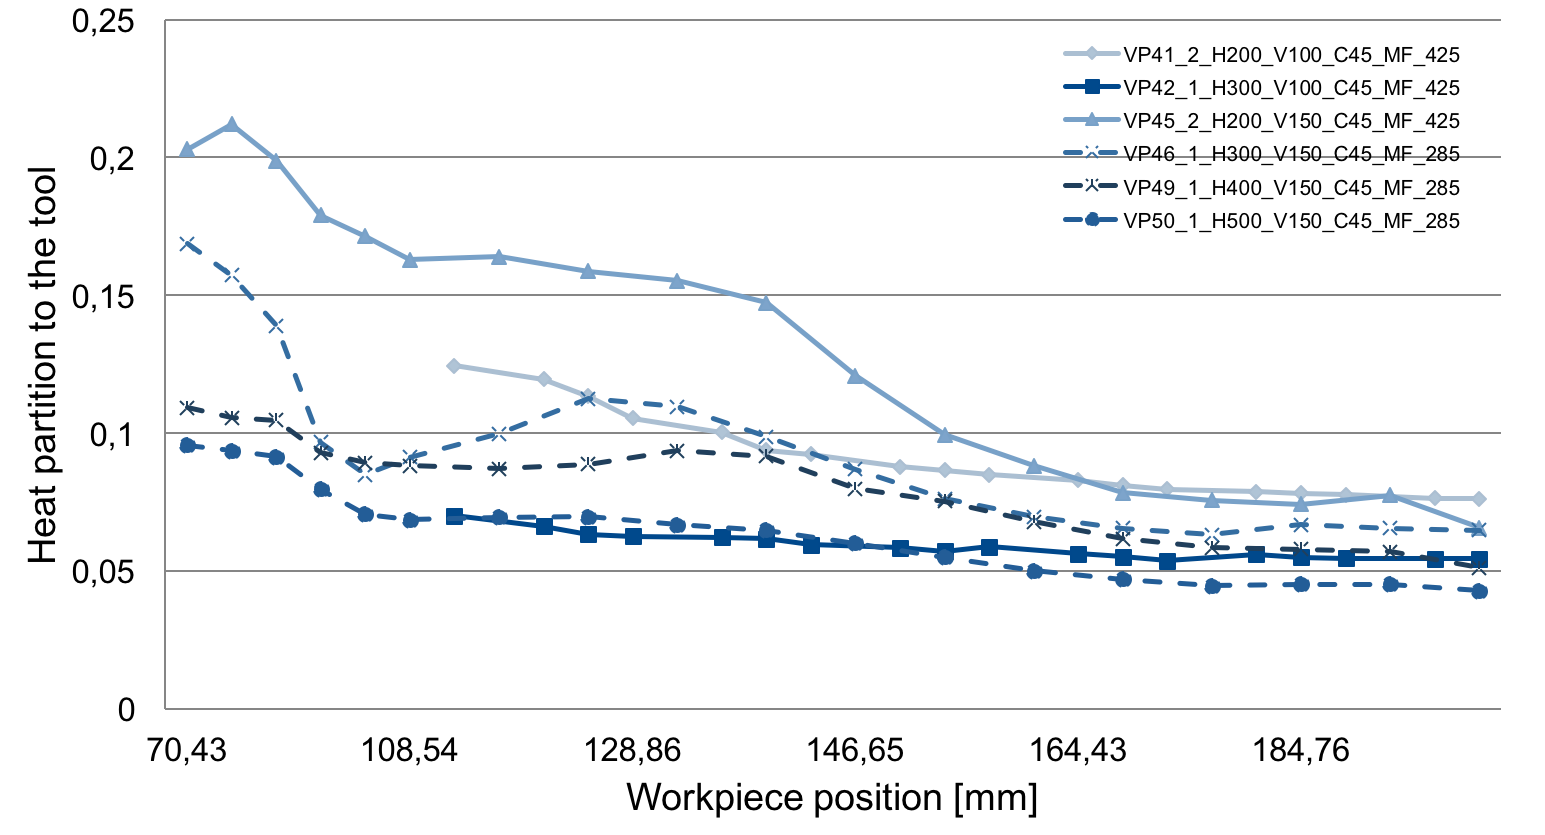
\includegraphics[scale=0.55]{Imagens/partTool.png}
		\caption{Heat partition ratio for tool}
		\label{fig:hpartTool}
	\end{figure}
